\section{Experiments}

\subsection{Introduction to the tools}
\subsubsection{Python (\texttt{regex})}
\texttt{regex} is the Python module intended to replace the \texttt{re} module
at some point. It is a fairly fully fletched Regex module, that also supports
approximate matching. Because of this and the ease of creating the necessary
scripts we chose to include it in the benchmarks.

\subsubsection{Approximate Kleenex}
Approximate matching was introduced to Kleenex by P. Troelsen in his masters
thesis~\cite{troelsen2016approximate}.

\subsubsection{Scan For Matches}
Scan For Matches is a approximate matching tool specifically for DNA matching.
It is written in C and has a bunch of DNA specific niceties that the other
tools don't, such as using FASTA files directly, and reverse complements
(matching a reversed and DNA complemented pattern).

\subsubsection{NR-grep}
NR-grep~\cite{navarro2001nr} is a fast pattern matching tool, similar to
\texttt{grep}, that also supports approximate matching.


\subsection{Experiment setup and benchmark description}
The experiments where run on the \texttt{gpu02} machine
\begin{description}
    \item[CPU] Intel Xeon E5-2650 v2 (2.60 GHz)
    \item[RAM] 128 GB
\end{description}

The data set used for the benchmark is from
\url{ftp://ftp-trace.ncbi.nih.gov/1000genomes/ftp/technical/reference/human_g1k_v37.fasta.gz}
and is 2.9 GBs uncompressed, for most of the benchmarks we used a file where we
stripped the newlines, so they would not count as an error, except for the
nrgrep trails since it could not handle lines longer than $2^{16}$.


\subsection{Results}

\begin{figure}[!ht]
  \centering
  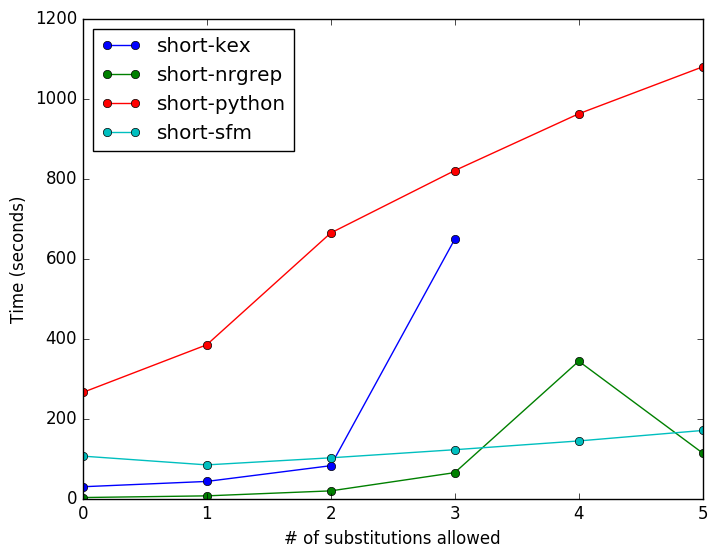
\includegraphics[width=0.9\textwidth]{images/short.png}
  \caption{Execution times for approximate Kleenex, NR-grep, Python's
    \texttt{regex} module, and \texttt{scan\_for\_matches}, when searching for
    the pattern \texttt{/TGCAAGCGTTAAT/<k>} for $k=0..5$.}
  \label{fig:short}
\end{figure}

\begin{figure}[!ht]
  \centering
  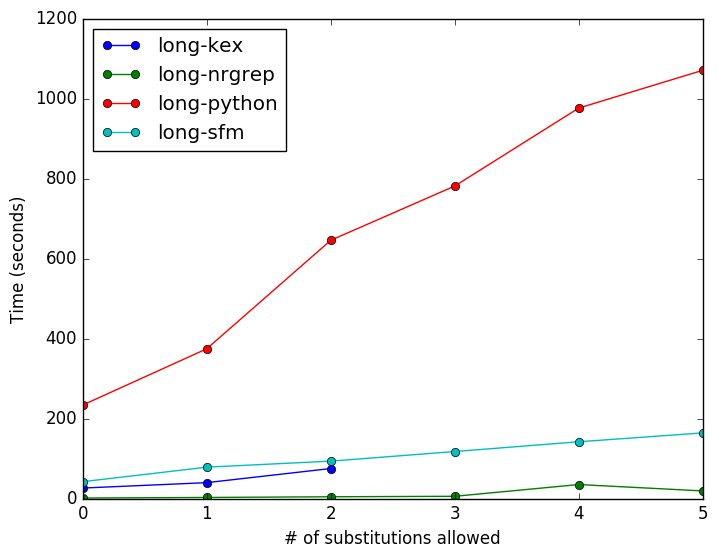
\includegraphics[width=0.9\textwidth]{images/long.png}
  \caption{Execution times for the evaluated tools when searching for the
    pattern \texttt{/GCCCAGAGAACTTTCAGGATGACACCAGCAAGG/<k>} for $k=0..5$.}
  \label{fig:long}
\end{figure}

\begin{figure}[!ht]
  \centering
  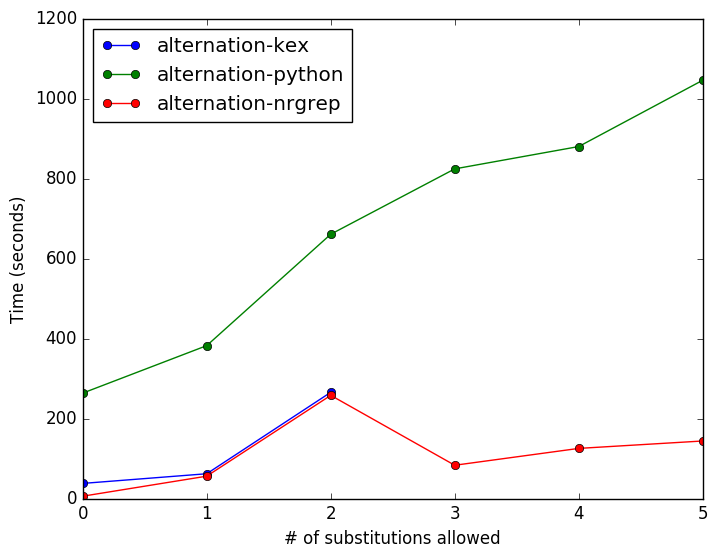
\includegraphics[width=0.9\textwidth]{images/alternation.png}
  \caption{Execution times for the evaluated tools when searching for the
    pattern \texttt{(/GCCCAGAGA/|/ACTTTCAGGA/)<k>} for $k=0..5$.}
  \label{fig:alternation}
\end{figure}

\begin{figure}[!ht]
  \centering
  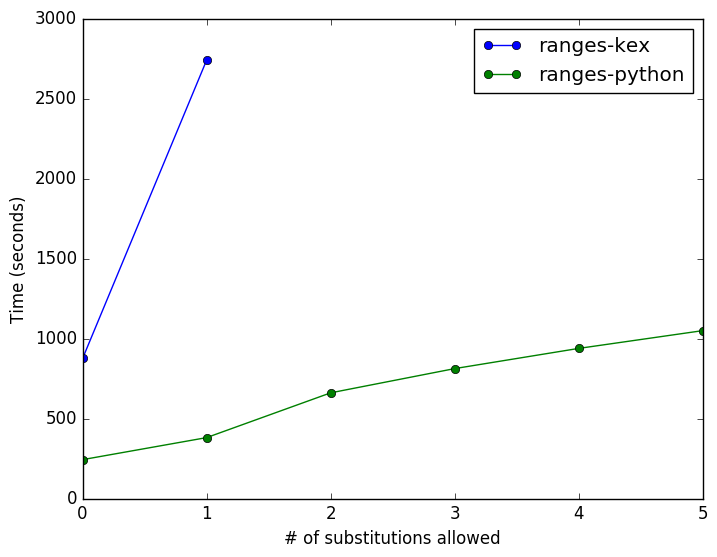
\includegraphics[width=0.9\textwidth]{images/ranges.png}
  \caption{Execution times for the evaluated tools when searching for the
    pattern \texttt{([ACGT]{5,15} /TGCAAGCGTTAAT/)<k>} for $k=0..5$.}
  \label{fig:ranges}
\end{figure}


%%% Local Variables:
%%% mode: latex
%%% TeX-master: "main"
%%% End:
